\documentclass[aspectratio=169]{beamer}

\usepackage[utf8]{inputenc}
\usetheme{Madrid}
\usecolortheme{beaver}
\usepackage{fontspec}
\usepackage{listings}
\usepackage{fancyvrb}
\usepackage{xcolor}

\hypersetup{
    colorlinks=true,
    linkcolor=blue,
    filecolor=magenta,
    urlcolor=blue,
    pdftitle={Test your Kubernetes operator with OLM},
    bookmarks=true,
    pdfpagemode=FullScreen,
}

\newcommand*{\fvtextcolor}[2]{\textcolor{#1}{#2}}

\title{Test your Kubernetes operator with OLM}
\author{Baiju Muthukadan \and Avni Sharma}
\date{May 15, 2019}
\logo{
\includegraphics[height=1.0cm]{images/Logo-RedHat-B-Color-RGB.png}}

\begin{document}
\beamertemplatenavigationsymbolsempty

\setmainfont
[ Path = ../fonts/,
UprightFont = DejaVuSerif.ttf,
ItalicFont = DejaVuSerif-Italic.ttf,
BoldFont = DejaVuSerif-Bold.ttf,
BoldItalicFont = DejaVuSerif-BoldItalic.ttf,
Numbers={Lining, Monospaced},
] {DejaVu Serif}

\setsansfont
[ Path = ../fonts/,
UprightFont = DejaVuSans.ttf,
ItalicFont = DejaVuSans-Oblique.ttf,
BoldFont = DejaVuSans-Bold.ttf,
BoldItalicFont = DejaVuSans-BoldOblique.ttf,
Numbers={Lining, Monospaced},
] {DejaVu Sans}

\setmonofont
[ Path = ../fonts/,
UprightFont = DejaVuSansMono.ttf,
ItalicFont = DejaVuSansMono-Oblique.ttf,
BoldFont = DejaVuSansMono-Bold.ttf,
BoldItalicFont = DejaVuSansMono-BoldOblique.ttf,
Numbers={Lining, Monospaced},
] {DejaVu Sans Mono}


\newfontfamily{\vollkorn}
[ Path = ../fonts/,
UprightFont = Vollkorn-Regular.otf,
ItalicFont = Vollkorn-Italic.otf,
BoldFont = Vollkorn-Bold.otf,
BoldItalicFont = Vollkorn-BoldItalic.otf,
Numbers={Lining, Monospaced},
] {Vollkorn}

\newfontfamily{\dejavuserif}
[ Path = ../fonts/,
UprightFont = DejaVuSerif.ttf,
ItalicFont = DejaVuSerif-Italic.ttf,
BoldFont = DejaVuSerif-Bold.ttf,
BoldItalicFont = DejaVuSerif-BoldItalic.ttf,
Numbers={Lining, Monospaced},
] {DejaVu Serif}

\newfontfamily{\dejavusans}
[ Path = ../fonts/,
UprightFont = DejaVuSans.ttf,
ItalicFont = DejaVuSans-Oblique.ttf,
BoldFont = DejaVuSans-Bold.ttf,
BoldItalicFont = DejaVuSans-BoldOblique.ttf,
Numbers={Lining, Monospaced},
] {DejaVu Sans}

\newfontfamily{\dejavumono}
[ Path = ../fonts/,
UprightFont = DejaVuSansMono.ttf,
ItalicFont = DejaVuSansMono-Oblique.ttf,
BoldFont = DejaVuSansMono-Bold.ttf,
BoldItalicFont = DejaVuSansMono-BoldOblique.ttf,
Numbers={Lining, Monospaced},
] {DejaVu Sans Mono}

\frame{\titlepage}

\begin{frame}
  \frametitle{About Us}

  \begin{itemize}
  \item \href{https://github.com/Avni-Sharma}{Baiju} is a Senior Software Engineer
  \item \href{https://github.com/baijum}{Avni} is an Associate Software Engineer
  \item Both of us work on DevConsole Operator
  \end{itemize}

\end{frame}

\begin{frame}
  \frametitle{Problem Statement}

  As a development team, we need to run end-to-end test for our
  operator.  To run end-to-end test, we need a mechanism to setup the
  infrastructure which includes the operator deployment and other
  dependent resources (CRDs, service account, role, and role binding).

\end{frame}

\begin{frame}
  \frametitle{Agenda}

  \begin{itemize}
  \item Introduction to Operator Framework
  \item Setting up resources through Operator Lifecycle Manager (OLM)
    for e2e testing
  \item Running e2e test through OpenShift CI
  \end{itemize}

\end{frame}

\begin{frame}
  \frametitle{DevConsole Operator}

  
\includegraphics[scale=.15]{images/Logo-Red_Hat-OpenShift_4-A-Standard-RGB.png}\\[.25in]

  Provides a developer-focused view in OpenShift 4

\end{frame}

\begin{frame}

  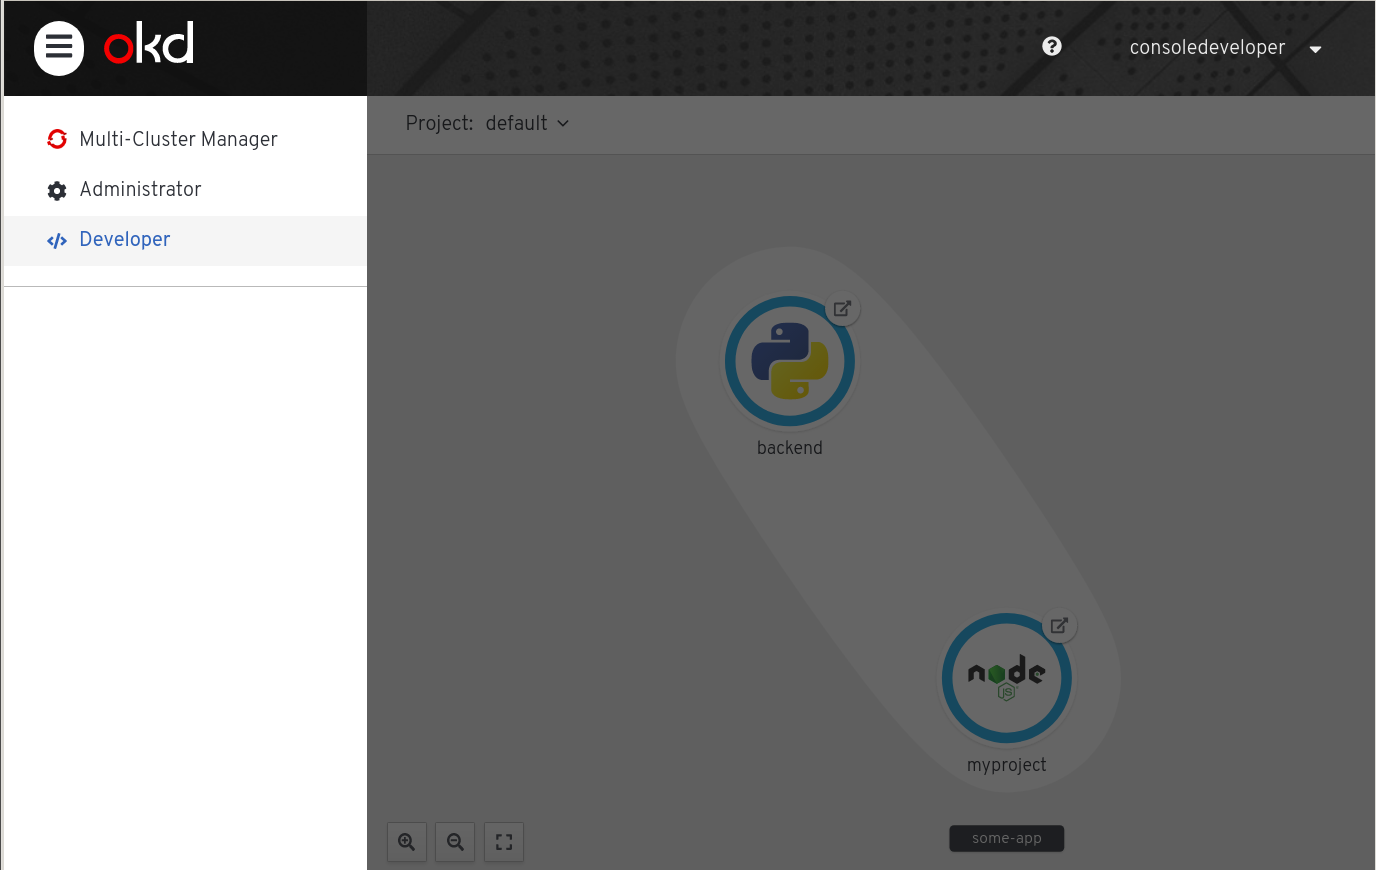
\includegraphics[scale=.25]{images/devconsole.png}

\end{frame}

\begin{frame}
  \frametitle{Operator Framework}

  
\includegraphics[scale=.50]{images/operator_logo_framework_color.png}

  A toolkit to manage Kubernetes native applications, called Operators.

\end{frame}

\begin{frame}
  \frametitle{Example Operators}

  \begin{itemize}
  \item \url{https://github.com/redhat-developer/devconsole-operator}
  \item \url{https://github.com/openshift/tektoncd-pipeline-operator}
  \item \url{https://github.com/operator-framework/operator-marketplace}
  \end{itemize}

\end{frame}

\begin{frame}
  \frametitle{Operator Framework Parts}

  
\includegraphics[scale=.50]{images/operator_logo_sdk_color.png}

  
\includegraphics[scale=.50]{images/operator_logo_lifecycle_manager_color.png}

  
\includegraphics[scale=.50]{images/operator_logo_metering_color.png}

  \url{https://github.com/operator-framework}

\end{frame}

\begin{frame}
  \frametitle{Operator Lifecycle Manager (OLM)}

  Oversees operator:
  \begin{itemize}
  \item Installation
  \item Updates
  \item Lifecycle
  \end{itemize}

\end{frame}

\begin{frame}
  \frametitle{OLM CRDs}
  \begin{itemize}
    \item {\bf catalogsources.operators.coreos.com}
    \item clusterserviceversions.operators.coreos.com
    \item installplans.operators.coreos.com
    \item operatorgroups.operators.coreos.com
    \item {\bf subscriptions.operators.coreos.com}
  \end{itemize}
\end{frame}


\begin{frame}

  \frametitle{Catalog Source}

  \begin{itemize}
  \item Repository of Cluster Service Version (CSV) files and CRDs
  \item Two types
    \begin{itemize}
    \item gRPC
    \item Internal (based on ConfigMap)
    \end{itemize}
  \item Public repository: \url{https://www.operatorhub.io}
  \end{itemize}

  To create a custom gRPC use this base image:\\
  quay.io/openshift/origin-operator-registry:latest

\end{frame}

\begin{frame}[fragile]

  \frametitle{File: manifests/devconsole/0.1.0/devconsole-operator.v0.1.0.clusterserviceversion.yaml}

  \begin{Verbatim}[fontsize=\small]
apiVersion: operators.coreos.com/v1alpha1
kind: ClusterServiceVersion
metadata:
  annotations:
    capabilities: Full Lifecycle
    description: The operator that enables a developer-focused perspective in OpenShift 4
    categories: "Developer Tools"
  name: devconsole-operator.v0.1.0
  namespace: placeholder
spec:
  apiservicedefinitions: {}
  customresourcedefinitions:

  ...
  \end{Verbatim}
\end{frame}

\begin{frame}[fragile]
  \frametitle{Manifests directory structure}

  \begin{Verbatim}[fontsize=\small]
manifests/
└── devconsole
    ├── 0.1.0
    │   ├── devconsole-operator.v0.1.0.clusterserviceversion.yaml
    │   ├── devconsole_v1alpha1_component_crd.yaml
    │   ├── devconsole_v1alpha1_gitsourceanalysis_crd.yaml
    │   └── devconsole_v1alpha1_gitsource_crd.yaml
    └── devconsole.package.yaml
  \end{Verbatim}

\end{frame}

\begin{frame}
  \begin{center}
    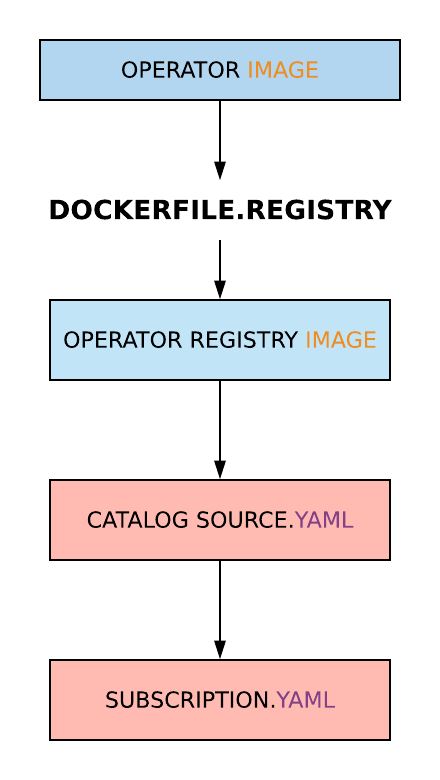
\includegraphics[scale=.50]{images/dockerfile.png}
  \end{center}
\end{frame}

\begin{frame}[fragile]
  \frametitle{Dockerfile to create registry}

  \begin{Verbatim}[fontsize=\small,commandchars=&\[\]]
FROM quay.io/openshift/origin-operator-registry:latest

ARG image=quay.io/redhat-developer/devconsole-operator
ARG version=0.1.0

COPY manifests manifests
COPY deploy/crds/*.yaml manifests/devconsole/${version}/

USER root
RUN sed -e "s,&fvtextcolor[red][REPLACE_IMAGE],${image}," -i
  manifests/devconsole/${version}/devconsole-operator.v${version}.
  &fvtextcolor[red][clusterserviceversion.yaml]
USER 1001

RUN initializer
CMD ["registry-server", "--termination-log=log.txt"]
  \end{Verbatim}

\end{frame}

\begin{frame}
  \begin{center}
    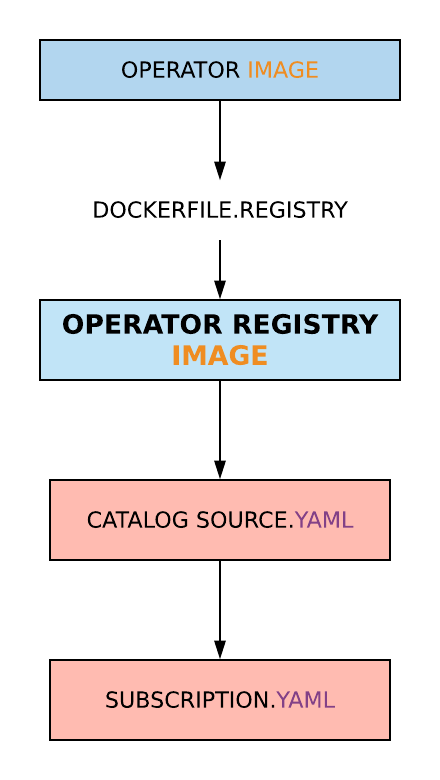
\includegraphics[scale=.50]{images/operator-registry.png}
  \end{center}
\end{frame}

\begin{frame}[fragile]
  \frametitle{Manifests directory structure}

  \begin{Verbatim}[fontsize=\small]
manifests/
└── devconsole
    ├── 0.1.0
    │   ├── devconsole-operator.v0.1.0.clusterserviceversion.yaml
    │   ├── devconsole_v1alpha1_component_crd.yaml
    │   ├── devconsole_v1alpha1_gitsourceanalysis_crd.yaml
    │   └── devconsole_v1alpha1_gitsource_crd.yaml
    └── devconsole.package.yaml
  \end{Verbatim}

\end{frame}

\begin{frame}
  \begin{center}
    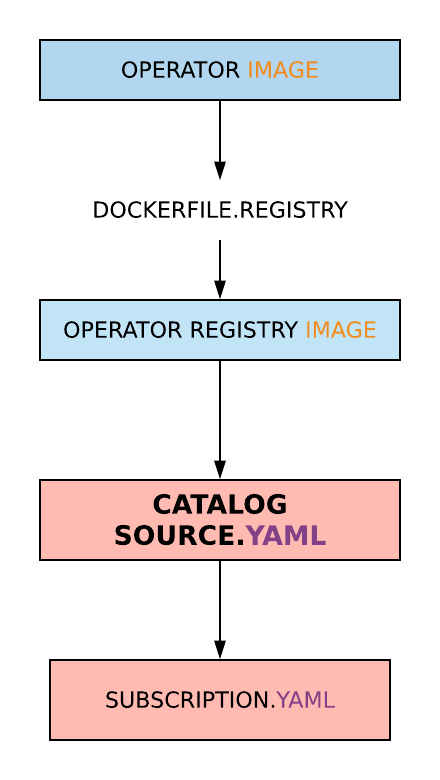
\includegraphics[scale=.50]{images/catalog.png}
  \end{center}
\end{frame}

\begin{frame}[fragile]
  \frametitle{CatalogSource}

  \begin{Verbatim}[fontsize=\small,commandchars=&\[\]]
# Ref. https://github.com/operator-framework/operator-lifecycle-manager
apiVersion: operators.coreos.com/v1alpha1
kind: CatalogSource
metadata:
  name: my-catalog
  namespace: openshift-operator-lifecycle-manager
spec:
  sourceType: grpc
  image: &fvtextcolor[red][REPLACE_IMAGE]
  displayName: Community Operators
  publisher: Red Hat
  \end{Verbatim}
\end{frame}

\begin{frame}

  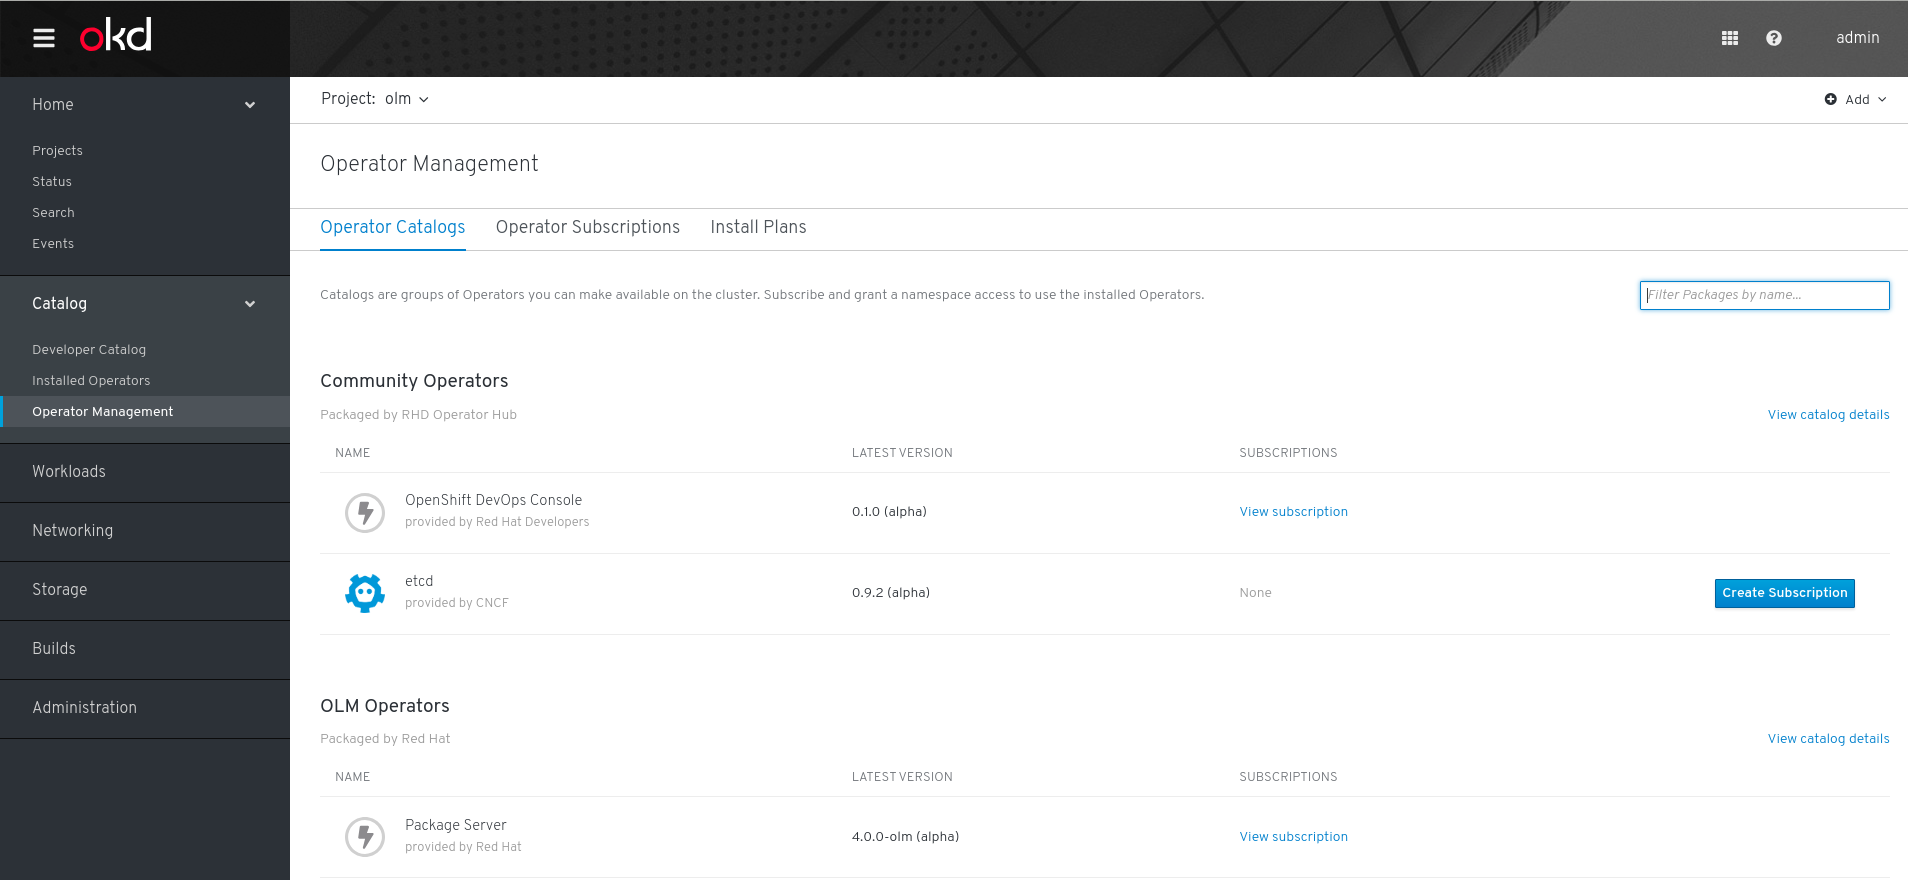
\includegraphics[scale=.20]{images/catsrc.png}

\end{frame}

\begin{frame}

  \frametitle{Subscription}

  Keep CSVs up to date by tracking a channel in a package.

\end{frame}

\begin{frame}[fragile]

  \frametitle{File: manifests/devconsole/devconsole.package.yaml}

  \begin{Verbatim}[fontsize=\small]
packageName: devconsole
channels:
- name: alpha
  currentCSV: devconsole-operator.v0.1.0
  \end{Verbatim}
\end{frame}

\begin{frame}
  \begin{center}
    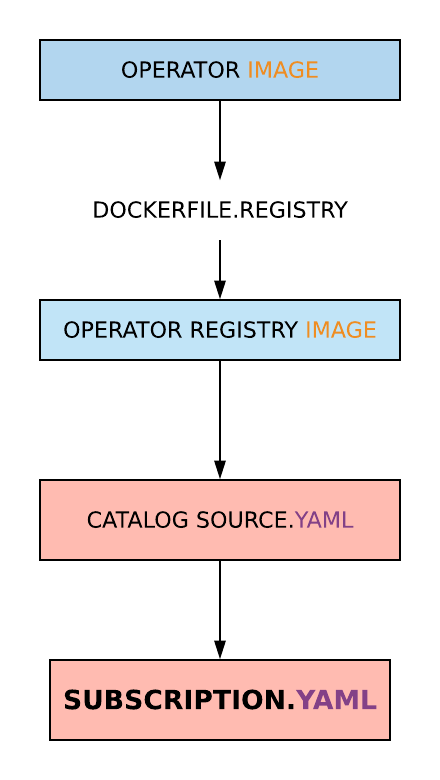
\includegraphics[scale=.50]{images/subscription2.png}
  \end{center}
\end{frame}

\begin{frame}[fragile]
  \frametitle{Subscription}

  \begin{Verbatim}[fontsize=\small]
# Ref. https://github.com/operator-framework/operator-lifecycle-manager
apiVersion: operators.coreos.com/v1alpha1
kind: Subscription
metadata:
  name: my-devconsole
  namespace: openshift-operators
spec:
  channel: alpha
  name: devconsole
  source: my-catalog
  sourceNamespace: openshift-operator-lifecycle-manager
  \end{Verbatim}
\end{frame}

\begin{frame}

  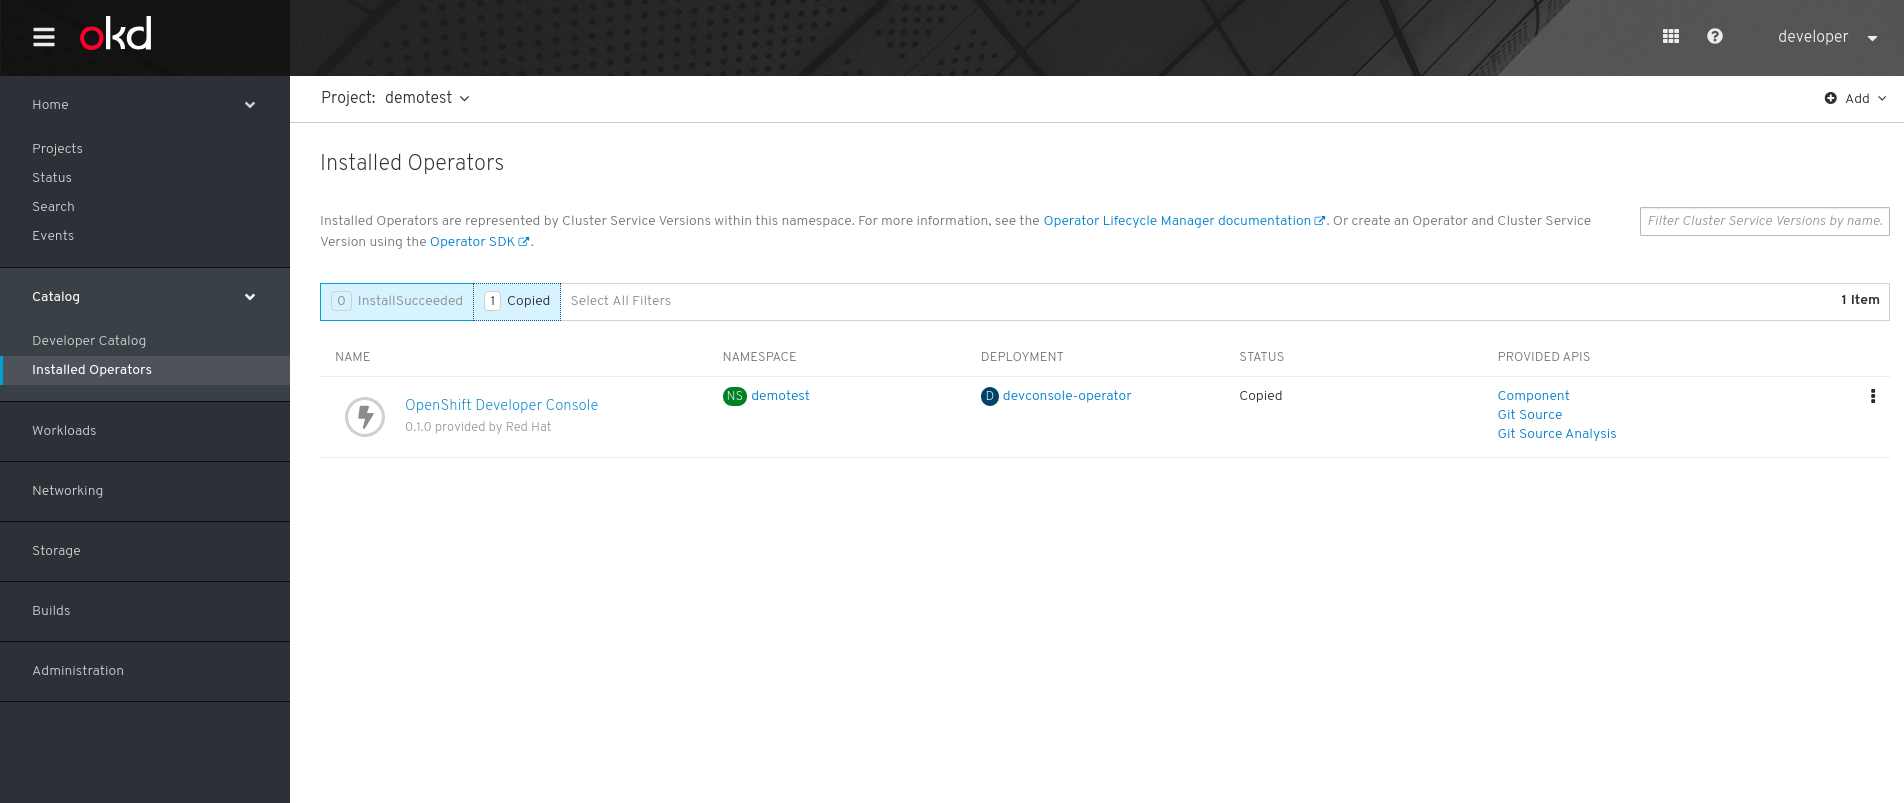
\includegraphics[scale=.20]{images/subscription.png}

\end{frame}

\begin{frame}

  \frametitle{OpenShift CI}

  \begin{itemize}
  \item OpenShift CI automates and simplifies the process of building and testing OpenShift component images
  \item OpenShift CI is run using ci-operator (This is {\bf not} a Kubernetes operator)
  \item ci-operator is built using Kubernetes prow
  \end{itemize}

\end{frame}

\begin{frame}[fragile]
  \frametitle{Setup operator resources without OLM}
  \begin{itemize}
  \item Create a temporary namespace/project
  \item Create all the CRDs
  \item Create service account
  \item Create role
  \item Create role binding
  \item Run the test
  \end{itemize}
\end{frame}

\begin{frame}[fragile]
  \frametitle{Setup operator resources without OLM}

  \begin{Verbatim}[fontsize=\small,commandchars=&\[\]]
.PHONY: test-e2e-ci
test-e2e-ci: get-test-namespace ./vendor
  $(Q)oc new-project $(TEST_NAMESPACE)
  $(Q)-oc apply -f ./deploy/crds/devconsole_v1alpha1_component_crd.yaml
  $(Q)-oc apply -f ./deploy/crds/devconsole_v1alpha1_gitsource_crd.yaml
  $(Q)-oc apply -f ./deploy/crds/devconsole_v1alpha1_gitsourceanalysis_crd.yaml
  $(Q)-oc apply -f ./deploy/service_account.yaml --namespace $(TEST_NAMESPACE)
  $(Q)-oc apply -f ./deploy/role.yaml --namespace $(TEST_NAMESPACE)
  $(Q)sed -e 's|REPLACE_NAMESPACE|$(TEST_NAMESPACE)|g' ./deploy/test/role_binding_test.yaml | oc apply -f -
  $(Q)sed -e 's|&fvtextcolor[red][REPLACE_IMAGE]|registry.svc.ci.openshift.org/$
    {OPENSHIFT_BUILD_NAMESPACE}/stable:devconsole-operator|g'
    ./deploy/test/&fvtextcolor[red][operator_test.yaml] | oc apply -f - --namespace $(TEST_NAMESPACE)
  $(eval DEPLOYED_NAMESPACE := $(TEST_NAMESPACE))
  $(Q)operator-sdk test local ./test/e2e --namespace
    $(TEST_NAMESPACE) --no-setup --go-test-flags "-v -timeout=15m"
  \end{Verbatim}
\end{frame}

\begin{frame}[fragile]
  \frametitle{Setup operator resources with OLM}
  \begin{itemize}
  \item Create catalog source
  \item Create subscription
  \item Run the test
  \end{itemize}
\end{frame}

\begin{frame}[fragile]
  \frametitle{Setup operator resources with OLM}

  \begin{Verbatim}[fontsize=\small,commandchars=&\[\]]
.PHONY: test-e2e-olm-ci
test-e2e-olm-ci: ./vendor
  $(Q)sed -e "s,&fvtextcolor[red][REPLACE_IMAGE],registry.svc.ci.openshift.org/
    ${OPENSHIFT_BUILD_NAMESPACE}/stable:devconsole-operator-registry,"
    ./test/e2e/&fvtextcolor[red][catalog_source_OS4.yaml] | oc apply -f -
  $(Q)oc apply -f ./test/e2e/subscription_OS4.yaml
  $(Q)./hack/check-crds.sh
  $(Q)operator-sdk test local ./test/e2e --no-setup
    --go-test-flags "-v -timeout=15m"
  \end{Verbatim}
\end{frame}

\begin{frame}[fragile]
  \frametitle{OpenShift CI Configuration}

  \begin{Verbatim}[fontsize=\small]
base_images:
  operator-registry:
    name: "4.0"
    namespace: ocp
    tag: operator-registry
images:
- from: operator-registry
  dockerfile_path: openshift-ci/Dockerfile.registry.intermediate
  to: operator-registry-base
- from: operator-registry-base
  dockerfile_path: openshift-ci/Dockerfile.registry.build
  to: devconsole-operator-registry
tests:
- as: e2e-olm-ci
  commands: make test-e2e-olm-ci
  openshift_installer_src:
    cluster_profile: aws
  \end{Verbatim}
\end{frame}

\begin{frame}[fragile]
  \frametitle{File: openshift-ci/Dockerfile.registry.intermediate}

  \begin{Verbatim}[fontsize=\small]
FROM quay.io/openshift/origin-operator-registry:latest
  \end{Verbatim}
\end{frame}

\begin{frame}[fragile]
  \frametitle{File: openshift-ci/Dockerfile.registry.build}

  \begin{Verbatim}[fontsize=\small,commandchars=&\[\]]
FROM quay.io/openshift/origin-operator-registry:latest

ARG version=0.1.0

COPY manifests manifests
COPY deploy/crds/*.yaml manifests/devconsole/${version}/

RUN sed -e "s,&fvtextcolor[red][REPLACE_IMAGE],registry.svc.ci.openshift.org/
  ${OPENSHIFT_BUILD_NAMESPACE}/stable:devconsole-operator,"
  -i manifests/devconsole/${version}/devconsole-operator.v${version}
  &fvtextcolor[red][.clusterserviceversion.yaml]
RUN initializer

USER 1001
EXPOSE 50051
CMD ["registry-server", "--termination-log=log.txt"]
  \end{Verbatim}
\end{frame}

\begin{frame}
  \begin{center}
    {\huge Thank You!}\\[1cm]
    \url{https://github.com/redhat-developer/devconsole-operator}
  \end{center}
\end{frame}

\end{document}
